\documentclass{article}
\usepackage[utf8]{inputenc}
\usepackage[german]{babel}
\usepackage{graphicx}
\usepackage{float}

\graphicspath{ {./images/} }

\title{Entwicklung eines IR-Spektrometers}
\author{Noah Jutz}
\date{}

\begin{document}

\maketitle
\tableofcontents


\section{Einführung}

% Notizen
%%%%%%%%%%%
% Fraunhoferlinien in Verbindung mit Infrarot-Spektroskopie
% - Was sind die linien?
% - Entdeckung
%   - Fraunhofer
%     - Astronomische Fernrohre
%     - Dokumentation der Linien
%   - Bunsen, Kirchhoff
%     - Absorption der Elemente
% - Zusammenhang mit IR-Spektroskopie
%   - |Fraunhoferlinien                   |IR-Spektroskopie
%     |-----------------------------------|-----------------------------
%     |Sichtbares licht                   |Unsichtbares Infrarotlicht
%     |chem. Zusammensetzung von Sternen  |Nachweis von Moleküstrukturen
%     |absorption von licht v. Elementen  |absorption v. IR-Strahlung v. Elementen
%     |zerlegung von Sonnenlicht          |zerlegung von IR-Strahlung
% Was ist Infrarotspektroskopie?
% - Spektroskopie
% - Wellenbereich 800nm - 1mm
% - Molekulspektroskopie
% - FTIR-Spektrometer, dispersives Spektrometer
%%%%%%%%%%

% 1.1 Fraunhoferlinien

% 1.1.1 Was sind sie?
Die Fraunhoferlinien, erstmals entdeckt von Joseph Fraunhofer, sind ein grundlegender Baustein in der Physik. Diese sind Absorptionslinien, welche im Sonnenspektrum beobachtet wurden.

% 1.1.2 Entdeckung Fraunhofer
Fraunhofer dokumentierte 1814 sorgfältig über 570 dieser Linien. Mit seinen Ergebnissen konnte er hochwertige astronomische Fernrohre herstellen.

\begin{figure}[H]
    \centering
    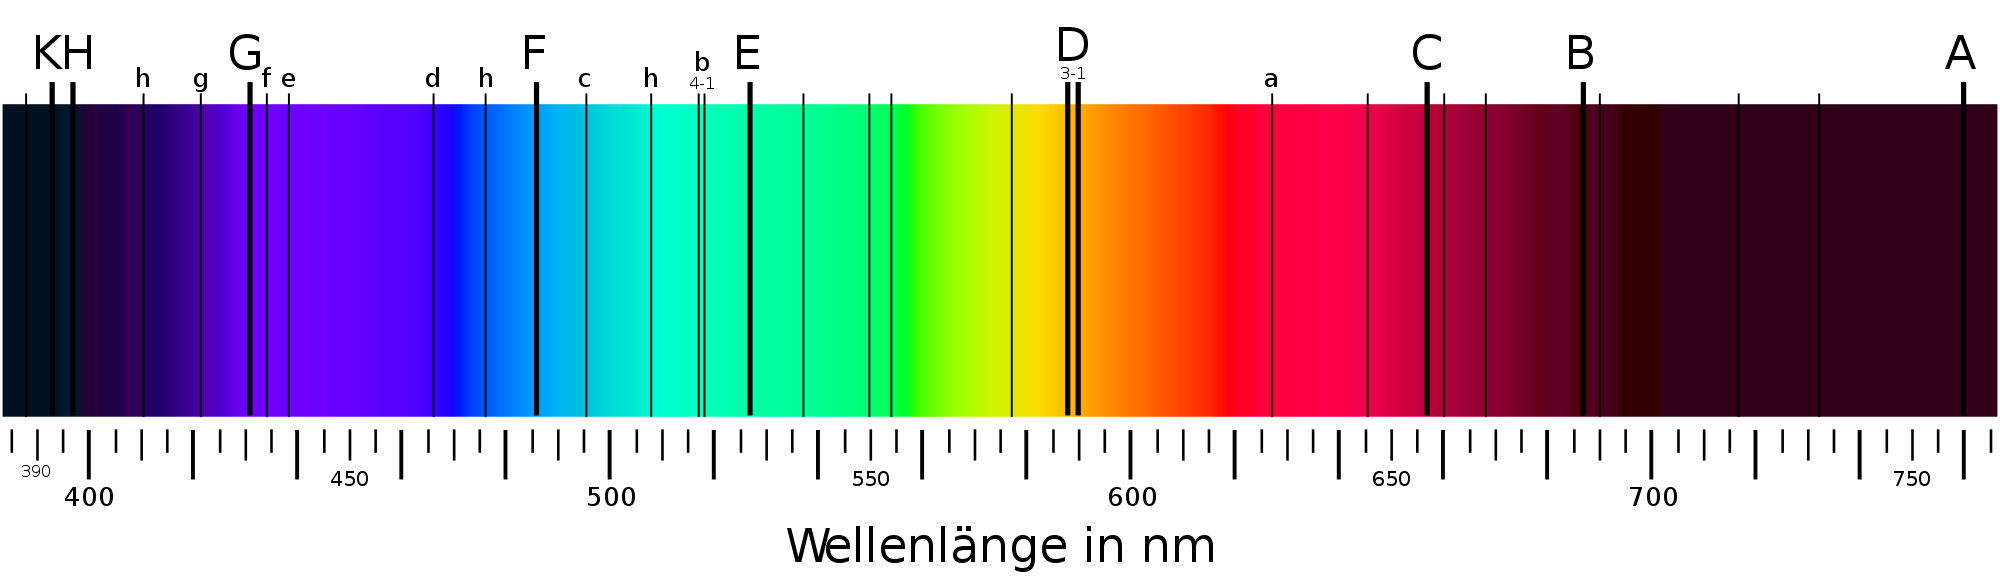
\includegraphics[width=0.8\textwidth]{2000px-Fraunhofer_lines_DE.svg.png}
    \caption{Fraunhoferlinien im Sonnenlichtspektrum}
\end{figure}

% 1.1.3 Entdeckung Bunsen, Kirchhoff
1859 führten Gustav Robert Kirchhoff und Robert Bunsen ein Experiment durch, bei dem eine Assoziazion zwischen chemischen Elementen und den Fraunhofer'schen Linien beobachtet wurde. Daraus folgt, dass die Absorptionslinien des Sonnenspektrums, welche Fraunhofer analysierte, die Absorptionseigenschaften dieser Elemente reflektiert.

\begin{table}[H]
    \centering
    \label{tab:wichtige-fraunhoferlinien}
    \begin{tabular}{l|l|l}
        Name & Element & Wellenlänge \\
        y    & $O_2$    & 898,765    \\
        Z    & $O_2$    & 822,696   
    \end{tabular}
    \caption{Wichtigste Fraunhoferlinien}
\end{table}

% 1.1.4 Zusammenhang IR-Spektroskopie

% 1.2 IR-Spektroskopie

% 1.2.1 Was ist es?

% 1.2.2 Zweck

% 1.2.3 FTIR-Spektrometer

% 1.2.4 Dispersives IR-Spektrometer

\section{Theoretische Grundlagen}

% Übergang

\subsection{Interferenz}

% Warum Grundlage?

\subsection{Doppelspaltexperiment}

% Warum Grundlage?
% Verbindung zu Interferenz

\subsection{Absorption}

% Warum Grundlage?

\section{IR-Spektrometer}

% Übergang

\subsection{Komponenten}

\subsubsection{Strahlquelle}

% λ × T = b
% Lötkolben

\subsubsection{Abbildende Optik}

% Spiegel

\subsubsection{Gitter}

% 600 Linien / mm
% Leypold
% Reflexionsgitter

\section{Versuch und Ergebnisse}

% b = k × λ ÷ sin(α)
%   α = 30°; λ = 530nm
%   -> b = 1500nm

\subsection{Versuchsaufbau}

% Bilder:
%   - loetkolben
%   - hg-lampe
%   - spiegel
%   - sensor
%   - gitter

\subsection{Ergebnisse}

% Diagramme
% Fehler

\section{Arduino} % Später

\subsection{Motorsteuerung}

\subsection{Signalerfassung}

\end{document}